\documentclass[11pt]{article}
\usepackage[a4paper,margin=22mm]{geometry}
\usepackage{amsmath,amssymb,graphicx,booktabs,longtable,array,pdflscape}
\usepackage[T1]{fontenc}
\usepackage[utf8]{inputenc}
\usepackage{hyperref,xcolor}
\hypersetup{colorlinks=true,linkcolor=blue!45!black,urlcolor=blue!45!black,citecolor=blue!45!black}
\setlength{\parindent}{0pt}
\setlength{\parskip}{5pt}
\setlength{\emergencystretch}{1em}
\newcommand{\code}[1]{\texttt{\detokenize{#1}}}
\newcolumntype{P}[1]{>{\raggedright\arraybackslash}p{#1}}
\newcommand{\panelpath}[1]{\href{https://github.com/bradlipovsky/zhu2020-fault-valving/blob/main/data/panels/#1.npz}{\nolinkurl{data/panels/#1.npz}}}

\pagestyle{myheadings}
\markright{INTERIM REPORT: incomplete reproduction study}
\title{Independent calculations of fault valving: interim results}
\author{Reproducibility study of Zhu, Allison, Dunham, and Yang (2020)}
\date{2026-10-09 00:47 UTC}
\begin{document}
\maketitle
\textbf{This is an interim scientific report. The full study remains incomplete.}
At this snapshot, 9 of 12 configured cases have completed, and 30 of 49 panel packages are available. Of these, 2 are independently reproduced constitutive-law panels and 28 are partial comparisons, including one newly drawn schematic. The 19 pending panels are labeled as not reproduced (pending) in the inventory; this describes their current availability, not a failed physical behavior. Pending runs are \texttt{baseline}, \texttt{baseline\_fine}, \texttt{baseline\_tight}. Their configured durations remain unchanged.

\section{Scope and independence}
Fault slip increases permeability, while healing between earthquakes restricts
drainage. The resulting pore-pressure changes alter frictional strength. We
independently implemented the coupled earthquake-cycle and fluid-flow model of
Zhu et al.~\cite{zhu} in C++. The scientific inputs are the published article,
its supplement, and comparable written model documentation. The earlier project
attempt used authors' archived outputs; that attempt and all its simulation
inputs are excluded here. No authors' code, simulation output, source dataset,
digitized output curve, or published image supplies a numerical result or figure
in this report. The schematic is newly drawn and is not a reproduced simulation.

Every displayed numerical panel comes from independent arrays in
\code{data/panels}. Its JSON sidecar records parameters, source hashes, selection
window, and provenance. A constitutive-law check establishes a narrower result
than recovery of an earthquake sequence. All displayed cycle calculations remain
partial comparisons because timing, event patterns, assumed inputs, or spatial
convergence remain unresolved. Published cycle durations below are approximate
visual readings used only as comparison targets, never computational inputs.
\section{Physical model and declared assumptions}
The elastic domain occupies $0\leq y\leq L_y$ and $0\leq z\leq L_z$, with depth
$z$ positive downward. Both dimensions are 500 km. Antiplane displacement $u$
is half the fault slip on $y=0$; the remote side is displaced at half the plate
rate. The top and bottom are traction free. The shear modulus is 32.4 GPa,
$V_p=10^{-9}$ m s$^{-1}$, and the radiation-damping coefficient is
$\eta_{\rm rad}=4.68\times10^6$ Pa s m$^{-1}$.

The regularized friction law and aging law are
\begin{align}
 f(V,\psi)&=a\,\operatorname{asinh}\!\left[\frac{V}{2V_0}
                     \exp\!\left(\frac{\psi}{a}\right)\right],\\
 \dot\psi&=\frac{b}{d_c}\left[V_0\exp\!\left(\frac{f_0-\psi}{b}\right)-|V|\right],\\
 \tau_{\rm qs}-\eta_{\rm rad}V&=(\sigma-p)f(V,\psi).
\end{align}
Here $V_0=10^{-6}$ m s$^{-1}$, $f_0=0.6$, and $d_c=2$ mm. Friction is signed;
slip speed is used in state and permeability evolution if reverse slip occurs.
This extends the paper's positive-sliding convention and is documented explicitly.
Radiation damping limits rapid slip within the quasi-dynamic approximation;
it does not reproduce propagating elastic waves.

Fault-zone fluid storage, Darcy flux, and permeability obey
\begin{align}
 n\beta\,\partial_t p&=\partial_z q,
 &q&=\frac{k}{\eta}\left(\partial_zp-\rho g\right),\\
 k&=k_{\min}+(k_*-k_{\min})\exp[-(\sigma-p)/\sigma_*],\\
 \dot k_*&=\frac{|V|}{L}(k_{\max}-k_*)-\frac{k_*-k_{\min}}{T}.
\end{align}
Positive $q$ denotes upward flow. The surface pressure is zero and the bottom
influx is fixed. We use $n\beta=10^{-11}$ Pa$^{-1}$, $\eta=10^{-4}$ Pa s,
$\rho=1000$ kg m$^{-3}$, $g=9.8$ m s$^{-2}$, $\sigma_*=30$ MPa, $L=1$ m,
$k_{\min}=10^{-19}$ m$^2$, and $k_{\max}=10^{-15}$ m$^2$.
The healing times are $10^7$, $10^8$, $10^9$, and $10^{10}$ s. Bottom influx is
$3\times10^{-9}$ m s$^{-1}$ except for $T=10^7$ s, where it is
$3.3\times10^{-10}$ m s$^{-1}$. Porosity changes, thermal pressurization, and
bulk poroelastic stress changes are omitted as in the published model.

Several inputs needed for an executable model are not fully specified in the
article or supplement. We assume $\sigma(z)=(22\,\mathrm{MPa}\,\mathrm{km}^{-1})z$,
consistent with the displayed normal-stress line in the original Fig. 1d.
We prescribe $a=0.01$ at the surface, increasing linearly to 0.03 at 15 km,
then increasing at $0.003$ km$^{-1}$. We set $a-b=-0.01$ above 13.5 km and
increase it linearly below that depth, crossing zero at 17 km. These profiles
continue to the bottom boundary. They approximate a parameter diagram, not a
digitized simulation result, and their exact agreement with the authors' inputs
cannot be established from the written record.

Initially $k_*$ has its steady-sliding value at $V_p$, and pressure is the
discrete steady solution with flux $q_0$ at every face. State is initialized at
its steady-sliding value at $V_p$. Initial velocity varies from $10^{-4}V_p$
above 17 km to $V_p$ below, through a hyperbolic tangent of width 1.5 km.
Elastic prestress balances that initial velocity. A Gaussian reduction of
$10^{-4}$ in $\psi$, centered at 12 km with width 1 km, perturbs the fault.
Earthquake times, rupture footprints, and subsequent slip are not prescribed.
These initial conditions are independent choices; no published restart is used.

An exploratory all-depth steady-sliding initialization was also tested.
Shallow elastic stiffness imposed a severe explicit time-step restriction.
The nearly locked shallow start is therefore used for the production runs;
its influence is assessed separately from numerical resolution. Full parameter
files and all choices are included in the repository.

\section{Independent numerical method}
The elastic boundary-value problem can be reduced analytically to a fault
stiffness operator. A cosine mode with $\kappa_j=j\pi/L_z$ has stiffness
\begin{equation}
 K_0=\frac{\mu}{2L_y},\qquad
 K_j=\frac{\mu\kappa_j}{2}\coth(\kappa_jL_y),\quad j>0.
\end{equation}
The factor one-half converts fault slip to one-sided displacement. These
eigenvalues retain the finite side and bottom boundaries. FFTW cosine transforms
apply this operator on cell centers, with $\tau_{\rm qs}=\tau_{\rm initial}-Kd$
and $d$ equal to accumulated slip minus $V_pt$.

Physical fault nodes form a graded subset of this auxiliary grid. If $P$
linearly interpolates physical slip to the cosine grid, the physical operator is
$W^{-1}P^T h K P$, where $W$ contains control-volume widths and $h$ is the
auxiliary spacing. This weighted Galerkin projection preserves constant traction,
elastic reciprocity, and positive elastic energy. It retains the fine grid
through the rupture region while reducing the number of far-depth unknowns.

Pressure is discretized by conservative finite volumes, using excess pressure
$p-\rho gz$ and harmonic face permeability. Gradients use actual node distances;
surface pressure is imposed at the surface and bottom flux enters storage directly.
This scheme differs from the paper's fourth-order summation-by-parts method.
The production cosine grid has 131,072 points, giving a minimum fault spacing
of 3.815 m. Spacing is finest through the rupture depths and down to 30 km;
it increases at greater depths toward a 1 km target. The final interval can
reach about 1.5 times that target to avoid an undersized boundary interval.
The surface spacing is about
eight times the minimum and decreases to the minimum over the upper 2 km.
Both the minimum and maximum spacings halve or double in refinement cases.
The number of physical nodes and the resolved frictional length scales are
recorded in the completed-case audit files. No stress or velocity floor replaces spatial resolution.

We use the fourth-order additive Runge--Kutta method ARK4(3)6L[2]SA\ \cite{kennedy},
treating fluid flow implicitly and slip, state, and $k_*$ explicitly. The nonlinear pressure
solve iterates permeability and a tridiagonal solve to an absolute pressure-update
tolerance of 0.001 Pa. An embedded third-order estimate controls errors in slip,
state, permeability, and pressure. The fourth-order solution is accepted. Production tolerance is
$10^{-5}$ in the scaled maximum norm; the time-accuracy case uses
$2.5\times10^{-6}$. A controlled interseismic benchmark showed that this tighter
tolerance reduced accumulated errors without substantially increasing the cost
of the graded calculation. The maximum step is $10^6$ s. Detailed coefficients, scales,
boundary formulas, and data formats are given in \code{documentation/numerics.md}.


\section{Completed runs and quantitative comparisons}
Every completed case passed an audit of all accepted history rows and saved
field profiles, including samples outside the figure windows. The audit checks
finite values, positive effective stress, permeability bounds, accepted error
estimates, consecutive steps, field/history consistency, and source and parameter
hashes. Fixed-pressure cases also retain pressure throughout their saved profiles.
These checks establish internal consistency; they do not establish sequence
convergence or agreement with the paper. The audit files are
\code{data/<case>/output_verification.json}.

\begin{center}\small
\begin{tabular}{lrrrr}\toprule
Case & Duration (yr) & Accepted steps & Profiles & Large events\\\midrule
reference & 400 & 164586 & 14041 & 5\\
short & 200 & 272347 & 8873 & 4\\
long & 350 & 306854 & 17162 & 6\\
long\_reference & 350 & 209873 & 12897 & 4\\
verylong & 500 & 216379 & 18414 & 3\\
verylong\_reference & 500 & 334274 & 19194 & 4\\
baseline\_coarse & 200 & 438564 & 14838 & 7\\
initialization & 100 & 282753 & 7219 & 4\\
normal\_stress & 100 & 287400 & 7227 & 4\\
\bottomrule\end{tabular}\end{center}
A seismic interval is a whole-fault maximum speed excursion above
$10^{-3}$ m s$^{-1}$. A resolved rupture accumulates at least 1 cm of slip in a
connected depth interval. A large event has a connected footprint reaching above
2 km and spanning more than 10 km. Slip is measured between the saved first-above
and first-below threshold profiles. Incomplete events cannot define cycles.
Velocity maps use the last complete large-event cycle; cumulative-slip profiles
use the last two complete cycles. All available recurrence intervals are retained
in each analysis file. Neither event selection nor time windows are fitted to
the published images.

\begin{center}\small
\begin{tabular}{lrrrr}\toprule
Case & Last cycle (yr) & All-cycle median (yr) & Paper (yr) & Difference (\%)\\\midrule
reference & 64 & 66 & 50 & 27.9\\
long\_reference & 88.4 & 88.4 & 160 & -44.8\\
long & 70.5 & 63.6 & 65 & 8.4\\
verylong\_reference & 95.1 & 95.2 & 160 & -40.6\\
verylong & 174 & 179 & 150 & 16.3\\
\bottomrule\end{tabular}\end{center}
The reference target is main Fig. 2a; the long-healing targets are supplementary
Figs. 3a,c and 5a,c. The differences describe the selected final cycles and do not
imply stationary recurrence. In particular, the two long-healing fixed-pressure
references differ substantially from their approximately 160-year targets.
Uncertain friction profiles and initialization, finite simulated duration, and
unestablished spatial convergence prevent assigning these discrepancies to one
cause. No high-healing-time mesh study has been completed.

\begin{center}\small
\begin{tabular}{lrrrr}\toprule
Case & $T$ (s) & $\Delta(\sigma-p)$ at 10 km (MPa) & Leading front & Deepest front\\
 & & & (m/yr) & (m/yr)\\\midrule
short & 1e+07 & 4.57 & 1.84e+03 & 1.53e+03\\
long & 1e+09 & 16.5 & 187 & 242\\
verylong & 1e+10 & 6.82 & 168 & 168\\
\bottomrule\end{tabular}\end{center}
The stress range uses the nearest saved depth, about 10.004 km. Front rates are
medians of all retained upward segments of the $|V|=V_p$ contour, with $R^2\geq0.8$,
at 13--20 km depth. The leading and deepest branches are contour extrema, not
tracked identities of individual pulses. Their definitions need not coincide
with the paper's reported migration speeds of 2500, 120, and 30 m/yr for these
three cases. The discrepancies are retained rather than selecting the branch
closest to the published rate.

The short-healing case produces aseismic pulses. The following medians compare
with the article's approximate one-year duration, few-year recurrence, and
few-centimeter slip scales. Pulse widths depend on our declared
threshold, $|V|\geq1.1V_p$. Each counted episode lasts at least 0.01 yr, lies
within the selected window, and remains below the seismic threshold at every
accepted whole-fault history sample. All qualifying episodes are retained in
the case analysis. The depth dependence limits any claim of agreement.
\begin{center}\small
\begin{tabular}{rrrrr}\toprule
Depth (km) & Episodes & Duration (yr) & Recurrence (yr) & Slip (cm)\\\midrule
15 & 14 & 0.302 & 3.04 & 4.72\\
18 & 11 & 0.611 & 3.17 & 2.46\\
20 & 2 & 0.894 & 8.64 & 3.19\\
\bottomrule\end{tabular}\end{center}

The final model assessment requires the baseline, mesh-refined case, and tighter
time-tolerance case together. This interim report does not treat completed
coarse-grid, normal-stress, or initialization runs as a completed sensitivity
comparison. Software fixtures and exploratory short calculations are excluded
from all scientific figures here.

\section{Panel inventory and provenance}
Each row specifies the original label, quantity, documentation, independent-data
command, plotting command, status, and discrepancy. Data paths follow
\code{data/panels/<label>.npz}, with parameters and provenance in the adjacent
JSON file. Commands are intended for a clean checkout or completed cases; do not
start a duplicate simulation in a directory containing a live run.
Supplementary Fig. 2 visibly labels rows a and b; its caption also mentions c
and d, which are not separately visible. The inventory therefore includes the
two displayed rows and records that inconsistency.
\begin{landscape}\scriptsize
\setlength{\tabcolsep}{3pt}
\begin{longtable}{P{10mm}P{30mm}P{34mm}P{39mm}P{32mm}P{23mm}P{65mm}}
\toprule Panel & Quantity & Documentation & Data command & Plot command & Status & Discrepancy\\\midrule\endhead
F1a & Geometry schematic and assumed friction profiles & Main Fig. 1a; Eqs. (7)-(9); Table 1; a(z), b(z) are assumed & \texttt{python3 scripts/panel.py F1a -{}-data} & \texttt{python3 scripts/plot.py F1a} & partial & New schematic, not a simulation reproduction; friction profiles are declared approximations.\\[5pt]
F1b & Permeability versus effective normal stress & Main Eq. (3), Fig. 1b; Table 1 & \texttt{python3 scripts/panel.py F1b -{}-data} & \texttt{python3 scripts/plot.py F1b} & independently reproduced & Analytic laws agree with numerical limiting-case verification.\\[5pt]
F1c & Healing and slip-enhancement limiting solutions & Main Eq. (4), Fig. 1c; Table 1 & \texttt{python3 scripts/panel.py F1c -{}-data} & \texttt{python3 scripts/plot.py F1c} & independently reproduced & Analytic laws agree with numerical limiting-case verification.\\[5pt]
F1d & Steady pressure, stress, and permeability profiles & Main Eqs. (2)-(4), Fig. 1d; assumed normal-stress gradient & \texttt{python3 scripts/panel.py F1d -{}-data} & \texttt{python3 scripts/plot.py F1d} & partial & Normal stress gradient is assumed; steady Darcy balance is independently verified.\\[5pt]
F2a & Slip velocity in time and step coordinates & Main Fig. 2; main Eqs. (1)-(9), Table 1 & \texttt{python3 scripts/panel.py F2a -{}-data} & \texttt{python3 scripts/plot.py F2a} & partial & Last complete interval 64 yr versus approximately 50 yr in Main Fig. 2a (+28\%). All-interval median 66 yr. Initial state and friction profiles remain uncertain.\\[5pt]
F2b & Cumulative slip profiles & Main Fig. 2; main Eqs. (1)-(9), Table 1 & \texttt{python3 scripts/panel.py F2b -{}-data} & \texttt{python3 scripts/plot.py F2b} & partial & Last complete interval 64 yr versus approximately 50 yr in Main Fig. 2a (+28\%). All-interval median 66 yr. Initial state and friction profiles remain uncertain.\\[5pt]
F2c & Slip velocity in time and step coordinates & Main Fig. 2; main Eqs. (1)-(9), Table 1 & \texttt{python3 scripts/panel.py F2c -{}-data} & \texttt{python3 scripts/plot.py F2c} & not reproduced (pending) & Pending completed baseline calculation and final extraction; no result supplied in this snapshot.\\[5pt]
F2d & Cumulative slip profiles & Main Fig. 2; main Eqs. (1)-(9), Table 1 & \texttt{python3 scripts/panel.py F2d -{}-data} & \texttt{python3 scripts/plot.py F2d} & not reproduced (pending) & Pending completed baseline calculation and final extraction; no result supplied in this snapshot.\\[5pt]
F3a & Effective normal stress history & Main Fig. 3; main Eqs. (1)-(4), Table 1 & \texttt{python3 scripts/panel.py F3a -{}-data} & \texttt{python3 scripts/plot.py F3a} & not reproduced (pending) & Pending completed baseline calculation and final extraction; no result supplied in this snapshot.\\[5pt]
F3b & Effective normal stress depth profiles & Main Fig. 3; main Eqs. (1)-(4), Table 1 & \texttt{python3 scripts/panel.py F3b -{}-data} & \texttt{python3 scripts/plot.py F3b} & not reproduced (pending) & Pending completed baseline calculation and final extraction; no result supplied in this snapshot.\\[5pt]
F3c & Permeability history & Main Fig. 3; main Eqs. (1)-(4), Table 1 & \texttt{python3 scripts/panel.py F3c -{}-data} & \texttt{python3 scripts/plot.py F3c} & not reproduced (pending) & Pending completed baseline calculation and final extraction; no result supplied in this snapshot.\\[5pt]
F3d & Permeability depth profiles & Main Fig. 3; main Eqs. (1)-(4), Table 1 & \texttt{python3 scripts/panel.py F3d -{}-data} & \texttt{python3 scripts/plot.py F3d} & not reproduced (pending) & Pending completed baseline calculation and final extraction; no result supplied in this snapshot.\\[5pt]
F3e & Upward fluid flux history & Main Fig. 3; main Eqs. (1)-(4), Table 1 & \texttt{python3 scripts/panel.py F3e -{}-data} & \texttt{python3 scripts/plot.py F3e} & not reproduced (pending) & Pending completed baseline calculation and final extraction; no result supplied in this snapshot.\\[5pt]
F3f & Upward fluid flux depth profiles & Main Fig. 3; main Eqs. (1)-(4), Table 1 & \texttt{python3 scripts/panel.py F3f -{}-data} & \texttt{python3 scripts/plot.py F3f} & not reproduced (pending) & Pending completed baseline calculation and final extraction; no result supplied in this snapshot.\\[5pt]
F4a & Slip velocity versus time & Main Fig. 4; Eqs. (1)-(9); Table 1 & \texttt{python3 scripts/panel.py F4a -{}-data} & \texttt{python3 scripts/plot.py F4a} & not reproduced (pending) & Pending completed baseline calculation and final extraction; no result supplied in this snapshot.\\[5pt]
F4b & Slip velocity versus accepted step & Main Fig. 4; Eqs. (1)-(9); Table 1 & \texttt{python3 scripts/panel.py F4b -{}-data} & \texttt{python3 scripts/plot.py F4b} & not reproduced (pending) & Pending completed baseline calculation and final extraction; no result supplied in this snapshot.\\[5pt]
F4c & Effective normal stress & Main Fig. 4; Eqs. (1)-(9); Table 1 & \texttt{python3 scripts/panel.py F4c -{}-data} & \texttt{python3 scripts/plot.py F4c} & not reproduced (pending) & Pending completed baseline calculation and final extraction; no result supplied in this snapshot.\\[5pt]
F4d & Permeability & Main Fig. 4; Eqs. (1)-(9); Table 1 & \texttt{python3 scripts/panel.py F4d -{}-data} & \texttt{python3 scripts/plot.py F4d} & not reproduced (pending) & Pending completed baseline calculation and final extraction; no result supplied in this snapshot.\\[5pt]
F5a & Slip velocity versus time & Main Fig. 5; Eqs. (1)-(9); Table 1; T=1e7 s, q0=3.3e-10 m/s & \texttt{python3 scripts/panel.py F5a -{}-data} & \texttt{python3 scripts/plot.py F5a} & partial & Complete aseismic episodes above 1.1 Vp at 15/18/20 km: 14/11/2. Median intervals: 3.04, 3.17, 8.64 yr. Durations and slip are tabulated in the report; exact pulse sequence is not recovered.\\[5pt]
F5b & Slip velocity versus accepted step & Main Fig. 5; Eqs. (1)-(9); Table 1; T=1e7 s, q0=3.3e-10 m/s & \texttt{python3 scripts/panel.py F5b -{}-data} & \texttt{python3 scripts/plot.py F5b} & partial & Complete aseismic episodes above 1.1 Vp at 15/18/20 km: 14/11/2. Median intervals: 3.04, 3.17, 8.64 yr. Durations and slip are tabulated in the report; exact pulse sequence is not recovered.\\[5pt]
F5c & Effective normal stress & Main Fig. 5; Eqs. (1)-(9); Table 1; T=1e7 s, q0=3.3e-10 m/s & \texttt{python3 scripts/panel.py F5c -{}-data} & \texttt{python3 scripts/plot.py F5c} & partial & Complete aseismic episodes above 1.1 Vp at 15/18/20 km: 14/11/2. Median intervals: 3.04, 3.17, 8.64 yr. Durations and slip are tabulated in the report; exact pulse sequence is not recovered.\\[5pt]
F5d & Permeability & Main Fig. 5; Eqs. (1)-(9); Table 1; T=1e7 s, q0=3.3e-10 m/s & \texttt{python3 scripts/panel.py F5d -{}-data} & \texttt{python3 scripts/plot.py F5d} & partial & Complete aseismic episodes above 1.1 Vp at 15/18/20 km: 14/11/2. Median intervals: 3.04, 3.17, 8.64 yr. Durations and slip are tabulated in the report; exact pulse sequence is not recovered.\\[5pt]
F6 & Upward migration of the |V|=Vp contour & Main Fig. 6 and Discussion; reported rates 2.50, 0.38, 0.12, 0.03 km/year & \texttt{python3 scripts/panel.py F6 -{}-data} & \texttt{python3 scripts/plot.py F6} & not reproduced (pending) & Pending completed baseline calculation and final extraction; no result supplied in this snapshot.\\[5pt]
S1a & Slip velocity at 5, 10, 15, and 20 km & Supplementary Fig. 1; main Eqs. (1)-(9) & \texttt{python3 scripts/panel.py S1a -{}-data} & \texttt{python3 scripts/plot.py S1a} & not reproduced (pending) & Pending completed baseline calculation and final extraction; no result supplied in this snapshot.\\[5pt]
S1b & Permeability at 5, 10, 15, and 20 km & Supplementary Fig. 1; main Eqs. (1)-(9) & \texttt{python3 scripts/panel.py S1b -{}-data} & \texttt{python3 scripts/plot.py S1b} & not reproduced (pending) & Pending completed baseline calculation and final extraction; no result supplied in this snapshot.\\[5pt]
S1c & Upward flux at 5, 10, 15, and 20 km & Supplementary Fig. 1; main Eqs. (1)-(9) & \texttt{python3 scripts/panel.py S1c -{}-data} & \texttt{python3 scripts/plot.py S1c} & not reproduced (pending) & Pending completed baseline calculation and final extraction; no result supplied in this snapshot.\\[5pt]
S1d & Effective stress at 5, 10, 15, and 20 km & Supplementary Fig. 1; main Eqs. (1)-(9) & \texttt{python3 scripts/panel.py S1d -{}-data} & \texttt{python3 scripts/plot.py S1d} & not reproduced (pending) & Pending completed baseline calculation and final extraction; no result supplied in this snapshot.\\[5pt]
S2a & Alternative cycle: slip velocity in time and step coordinates & Visible panels a,b of Supplementary Fig. 2; caption additionally mentions absent c,d & \texttt{python3 scripts/panel.py S2a -{}-data} & \texttt{python3 scripts/plot.py S2a} & not reproduced (pending) & Pending completed baseline calculation and final extraction; no result supplied in this snapshot.\\[5pt]
S2b & Alternative cycle: slip velocity in time and step coordinates & Visible panels a,b of Supplementary Fig. 2; caption additionally mentions absent c,d & \texttt{python3 scripts/panel.py S2b -{}-data} & \texttt{python3 scripts/plot.py S2b} & not reproduced (pending) & Pending completed baseline calculation and final extraction; no result supplied in this snapshot.\\[5pt]
S3a & Slip velocity in time and step coordinates & Supplementary Fig. 3; main Eqs. (1)-(9), Table 1 & \texttt{python3 scripts/panel.py S3a -{}-data} & \texttt{python3 scripts/plot.py S3a} & partial & Last complete interval 88.4 yr versus approximately 160 yr in Supplementary Fig. 3a (-45\%). All-interval median 88.4 yr. Initial state and friction profiles remain uncertain.\\[5pt]
S3b & Cumulative slip profiles & Supplementary Fig. 3; main Eqs. (1)-(9), Table 1 & \texttt{python3 scripts/panel.py S3b -{}-data} & \texttt{python3 scripts/plot.py S3b} & partial & Last complete interval 88.4 yr versus approximately 160 yr in Supplementary Fig. 3a (-45\%). All-interval median 88.4 yr. Initial state and friction profiles remain uncertain.\\[5pt]
S3c & Slip velocity in time and step coordinates & Supplementary Fig. 3; main Eqs. (1)-(9), Table 1 & \texttt{python3 scripts/panel.py S3c -{}-data} & \texttt{python3 scripts/plot.py S3c} & partial & Last complete interval 70.5 yr versus approximately 65 yr in Supplementary Fig. 3c (+8\%). All-interval median 63.6 yr. Initial state and friction profiles remain uncertain.\\[5pt]
S3d & Cumulative slip profiles & Supplementary Fig. 3; main Eqs. (1)-(9), Table 1 & \texttt{python3 scripts/panel.py S3d -{}-data} & \texttt{python3 scripts/plot.py S3d} & partial & Last complete interval 70.5 yr versus approximately 65 yr in Supplementary Fig. 3c (+8\%). All-interval median 63.6 yr. Initial state and friction profiles remain uncertain.\\[5pt]
S4a & Effective normal stress history & Supplementary Fig. 4; main Eqs. (1)-(4), Table 1 & \texttt{python3 scripts/panel.py S4a -{}-data} & \texttt{python3 scripts/plot.py S4a} & partial & At 10 km, stress range 16.5 MPa and permeability ratio 9.64. The target is reduced valving with long healing; event sequence and mesh convergence remain uncertain.\\[5pt]
S4b & Effective normal stress depth profiles & Supplementary Fig. 4; main Eqs. (1)-(4), Table 1 & \texttt{python3 scripts/panel.py S4b -{}-data} & \texttt{python3 scripts/plot.py S4b} & partial & At 10 km, stress range 16.5 MPa and permeability ratio 9.64. The target is reduced valving with long healing; event sequence and mesh convergence remain uncertain.\\[5pt]
S4c & Permeability history & Supplementary Fig. 4; main Eqs. (1)-(4), Table 1 & \texttt{python3 scripts/panel.py S4c -{}-data} & \texttt{python3 scripts/plot.py S4c} & partial & At 10 km, stress range 16.5 MPa and permeability ratio 9.64. The target is reduced valving with long healing; event sequence and mesh convergence remain uncertain.\\[5pt]
S4d & Permeability depth profiles & Supplementary Fig. 4; main Eqs. (1)-(4), Table 1 & \texttt{python3 scripts/panel.py S4d -{}-data} & \texttt{python3 scripts/plot.py S4d} & partial & At 10 km, stress range 16.5 MPa and permeability ratio 9.64. The target is reduced valving with long healing; event sequence and mesh convergence remain uncertain.\\[5pt]
S4e & Upward fluid flux history & Supplementary Fig. 4; main Eqs. (1)-(4), Table 1 & \texttt{python3 scripts/panel.py S4e -{}-data} & \texttt{python3 scripts/plot.py S4e} & partial & At 10 km, stress range 16.5 MPa and permeability ratio 9.64. The target is reduced valving with long healing; event sequence and mesh convergence remain uncertain.\\[5pt]
S4f & Upward fluid flux depth profiles & Supplementary Fig. 4; main Eqs. (1)-(4), Table 1 & \texttt{python3 scripts/panel.py S4f -{}-data} & \texttt{python3 scripts/plot.py S4f} & partial & At 10 km, stress range 16.5 MPa and permeability ratio 9.64. The target is reduced valving with long healing; event sequence and mesh convergence remain uncertain.\\[5pt]
S5a & Slip velocity in time and step coordinates & Supplementary Fig. 5; main Eqs. (1)-(9), Table 1 & \texttt{python3 scripts/panel.py S5a -{}-data} & \texttt{python3 scripts/plot.py S5a} & partial & Last complete interval 95.1 yr versus approximately 160 yr in Supplementary Fig. 5a (-41\%). All-interval median 95.2 yr. Initial state and friction profiles remain uncertain.\\[5pt]
S5b & Cumulative slip profiles & Supplementary Fig. 5; main Eqs. (1)-(9), Table 1 & \texttt{python3 scripts/panel.py S5b -{}-data} & \texttt{python3 scripts/plot.py S5b} & partial & Last complete interval 95.1 yr versus approximately 160 yr in Supplementary Fig. 5a (-41\%). All-interval median 95.2 yr. Initial state and friction profiles remain uncertain.\\[5pt]
S5c & Slip velocity in time and step coordinates & Supplementary Fig. 5; main Eqs. (1)-(9), Table 1 & \texttt{python3 scripts/panel.py S5c -{}-data} & \texttt{python3 scripts/plot.py S5c} & partial & Last complete interval 174 yr versus approximately 150 yr in Supplementary Fig. 5c (+16\%). All-interval median 179 yr. Initial state and friction profiles remain uncertain.\\[5pt]
S5d & Cumulative slip profiles & Supplementary Fig. 5; main Eqs. (1)-(9), Table 1 & \texttt{python3 scripts/panel.py S5d -{}-data} & \texttt{python3 scripts/plot.py S5d} & partial & Last complete interval 174 yr versus approximately 150 yr in Supplementary Fig. 5c (+16\%). All-interval median 179 yr. Initial state and friction profiles remain uncertain.\\[5pt]
S6a & Effective normal stress history & Supplementary Fig. 6; main Eqs. (1)-(4), Table 1 & \texttt{python3 scripts/panel.py S6a -{}-data} & \texttt{python3 scripts/plot.py S6a} & partial & At 10 km, stress range 6.82 MPa and permeability ratio 1.77. The target is reduced valving with long healing; event sequence and mesh convergence remain uncertain.\\[5pt]
S6b & Effective normal stress depth profiles & Supplementary Fig. 6; main Eqs. (1)-(4), Table 1 & \texttt{python3 scripts/panel.py S6b -{}-data} & \texttt{python3 scripts/plot.py S6b} & partial & At 10 km, stress range 6.82 MPa and permeability ratio 1.77. The target is reduced valving with long healing; event sequence and mesh convergence remain uncertain.\\[5pt]
S6c & Permeability history & Supplementary Fig. 6; main Eqs. (1)-(4), Table 1 & \texttt{python3 scripts/panel.py S6c -{}-data} & \texttt{python3 scripts/plot.py S6c} & partial & At 10 km, stress range 6.82 MPa and permeability ratio 1.77. The target is reduced valving with long healing; event sequence and mesh convergence remain uncertain.\\[5pt]
S6d & Permeability depth profiles & Supplementary Fig. 6; main Eqs. (1)-(4), Table 1 & \texttt{python3 scripts/panel.py S6d -{}-data} & \texttt{python3 scripts/plot.py S6d} & partial & At 10 km, stress range 6.82 MPa and permeability ratio 1.77. The target is reduced valving with long healing; event sequence and mesh convergence remain uncertain.\\[5pt]
S6e & Upward fluid flux history & Supplementary Fig. 6; main Eqs. (1)-(4), Table 1 & \texttt{python3 scripts/panel.py S6e -{}-data} & \texttt{python3 scripts/plot.py S6e} & partial & At 10 km, stress range 6.82 MPa and permeability ratio 1.77. The target is reduced valving with long healing; event sequence and mesh convergence remain uncertain.\\[5pt]
S6f & Upward fluid flux depth profiles & Supplementary Fig. 6; main Eqs. (1)-(4), Table 1 & \texttt{python3 scripts/panel.py S6f -{}-data} & \texttt{python3 scripts/plot.py S6f} & partial & At 10 km, stress range 6.82 MPa and permeability ratio 1.77. The target is reduced valving with long healing; event sequence and mesh convergence remain uncertain.\\[5pt]
\bottomrule\end{longtable}\end{landscape}
\clearpage\begin{figure}[p]\centering
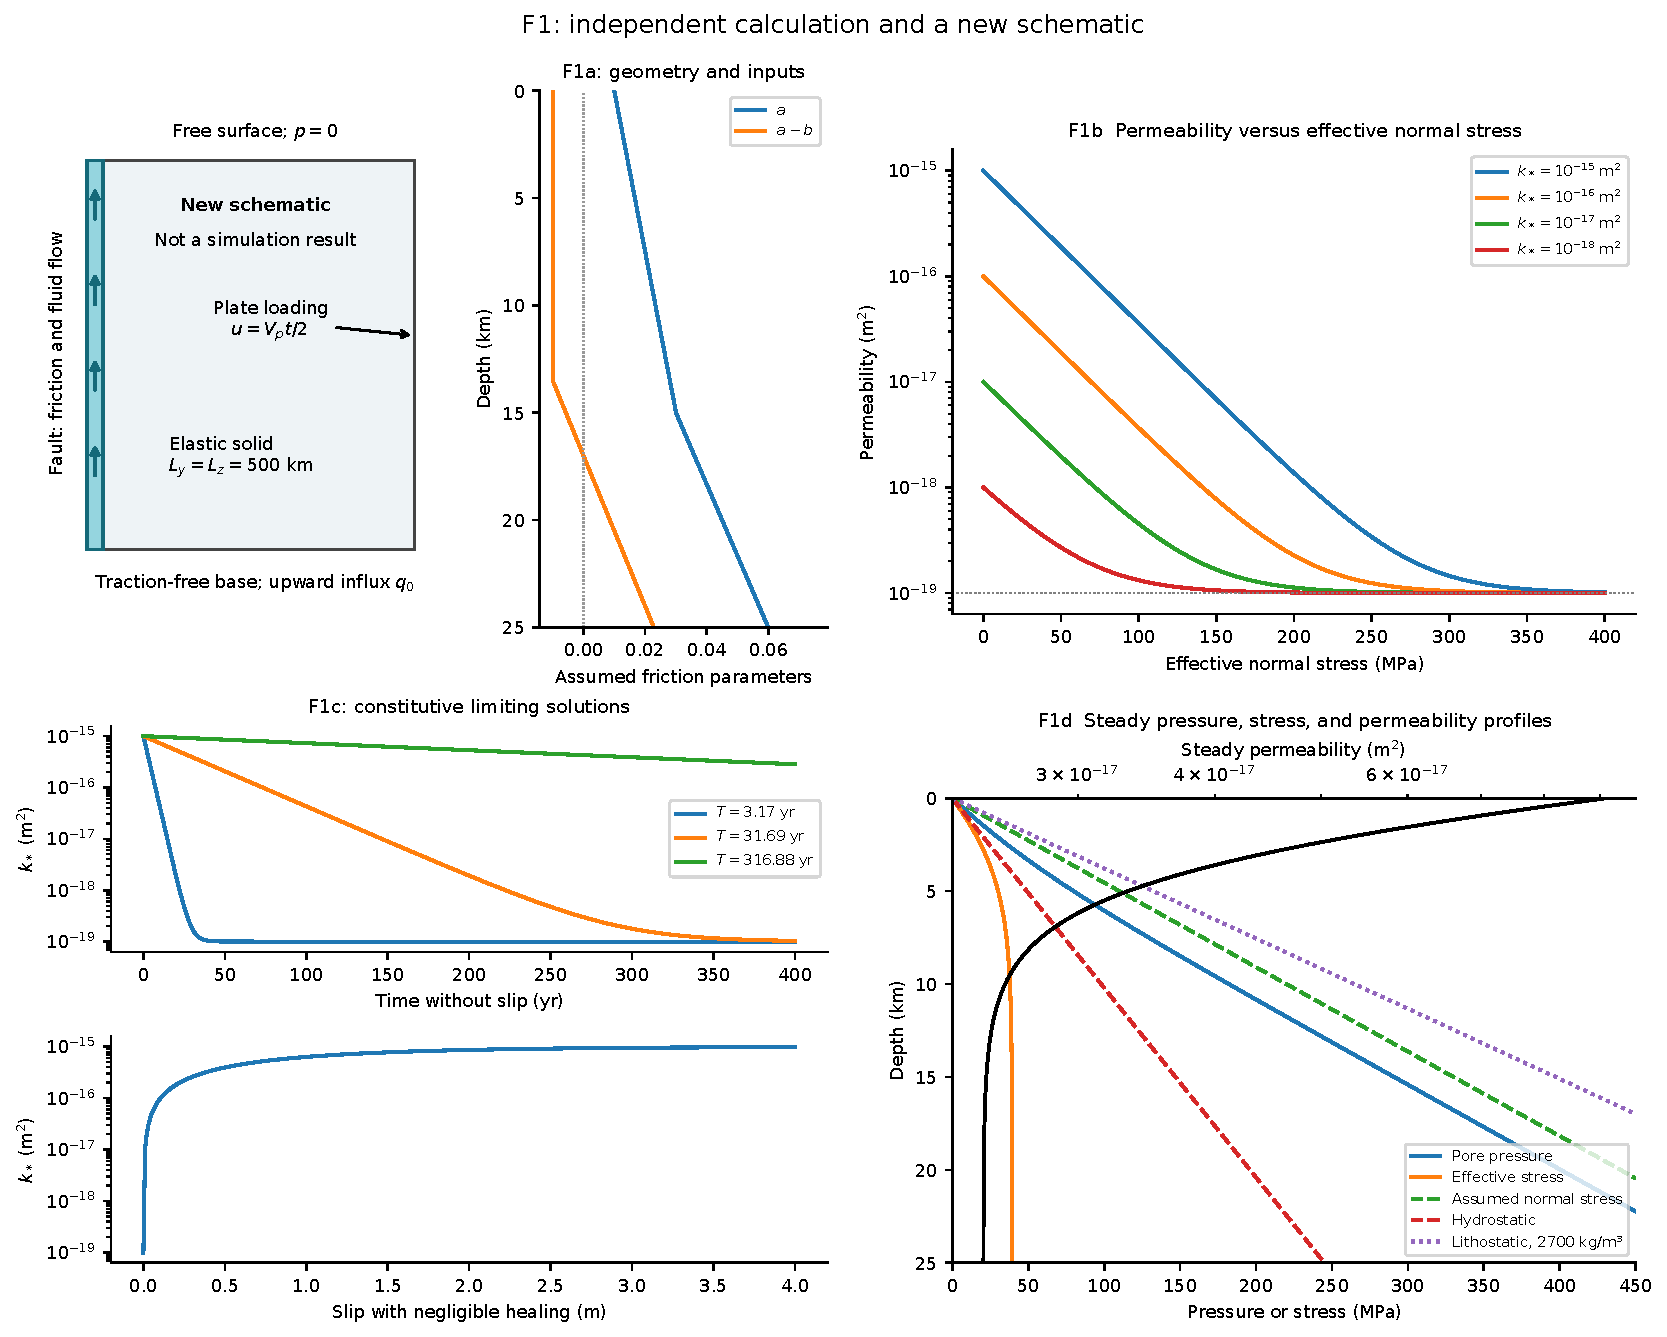
\includegraphics[width=\textwidth,height=.72\textheight,keepaspectratio]{../figures/F1.pdf}
\caption{Independent outputs corresponding to F1. F1a: Geometry schematic and assumed friction profiles; F1b: Permeability versus effective normal stress; F1c: Healing and slip-enhancement limiting solutions; F1d: Steady pressure, stress, and permeability profiles. Units and color scales are shown on the panels. Parameter files and selection rules are specified in the provenance sidecars. Panel F1a is a new schematic, not a simulated reproduction. Comparison target: Zhu et al.~\cite{zhu}.}\end{figure}
\clearpage\begin{figure}[p]\centering
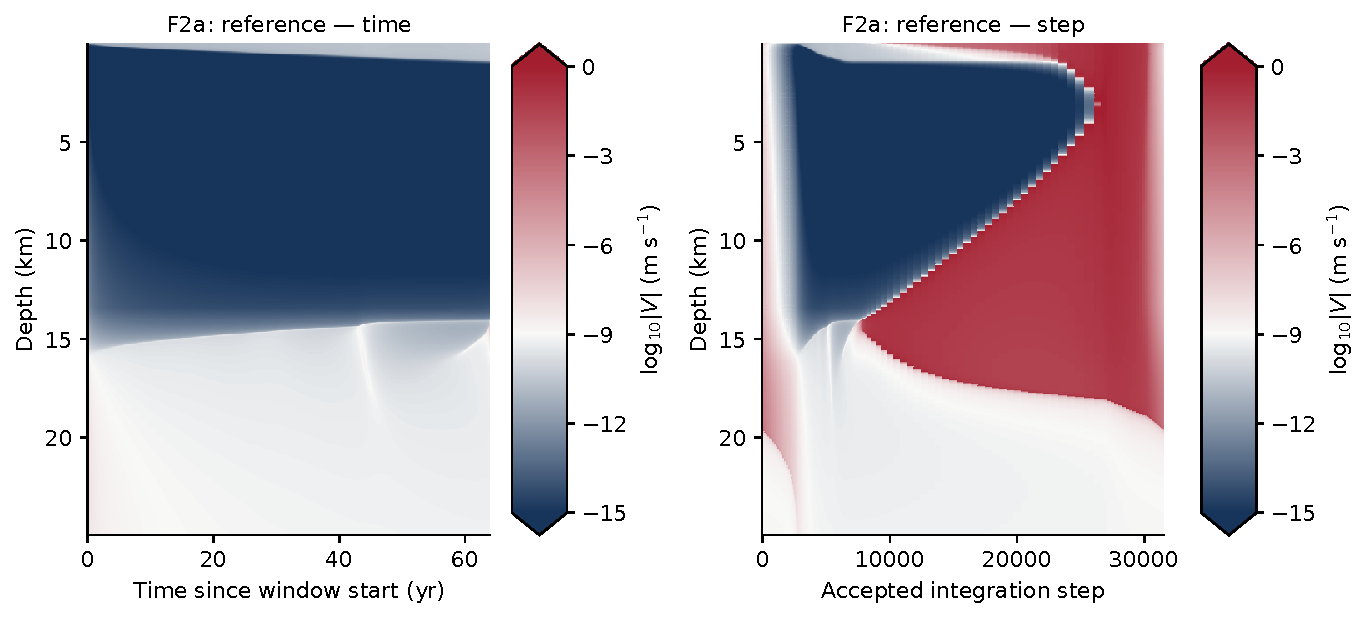
\includegraphics[width=\textwidth,height=.34\textheight,keepaspectratio]{../figures/panels/F2a.pdf}
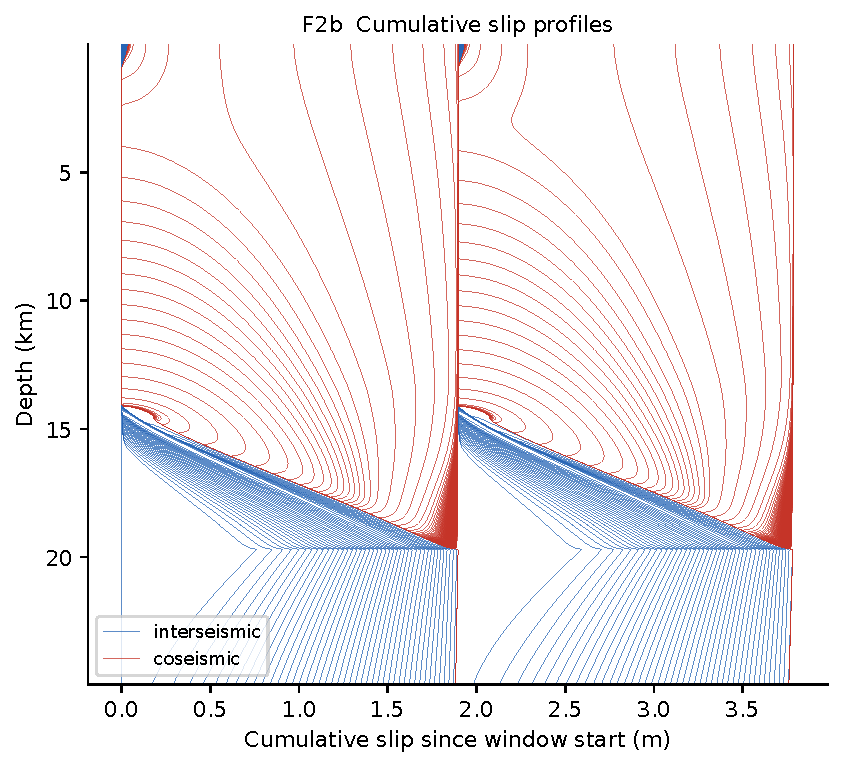
\includegraphics[width=\textwidth,height=.34\textheight,keepaspectratio]{../figures/panels/F2b.pdf}
\caption{Independent outputs corresponding to F2. F2a: Slip velocity in time and step coordinates; F2b: Cumulative slip profiles. Units and color scales are shown on the panels. Parameter files and selection rules are specified in the provenance sidecars. Pending and absent here: F2c, F2d. Cases: reference (T=1e+08 s; fixed pressure). These panels are partial comparisons. Comparison target: Zhu et al.~\cite{zhu}.}\end{figure}
\clearpage\begin{figure}[p]\centering
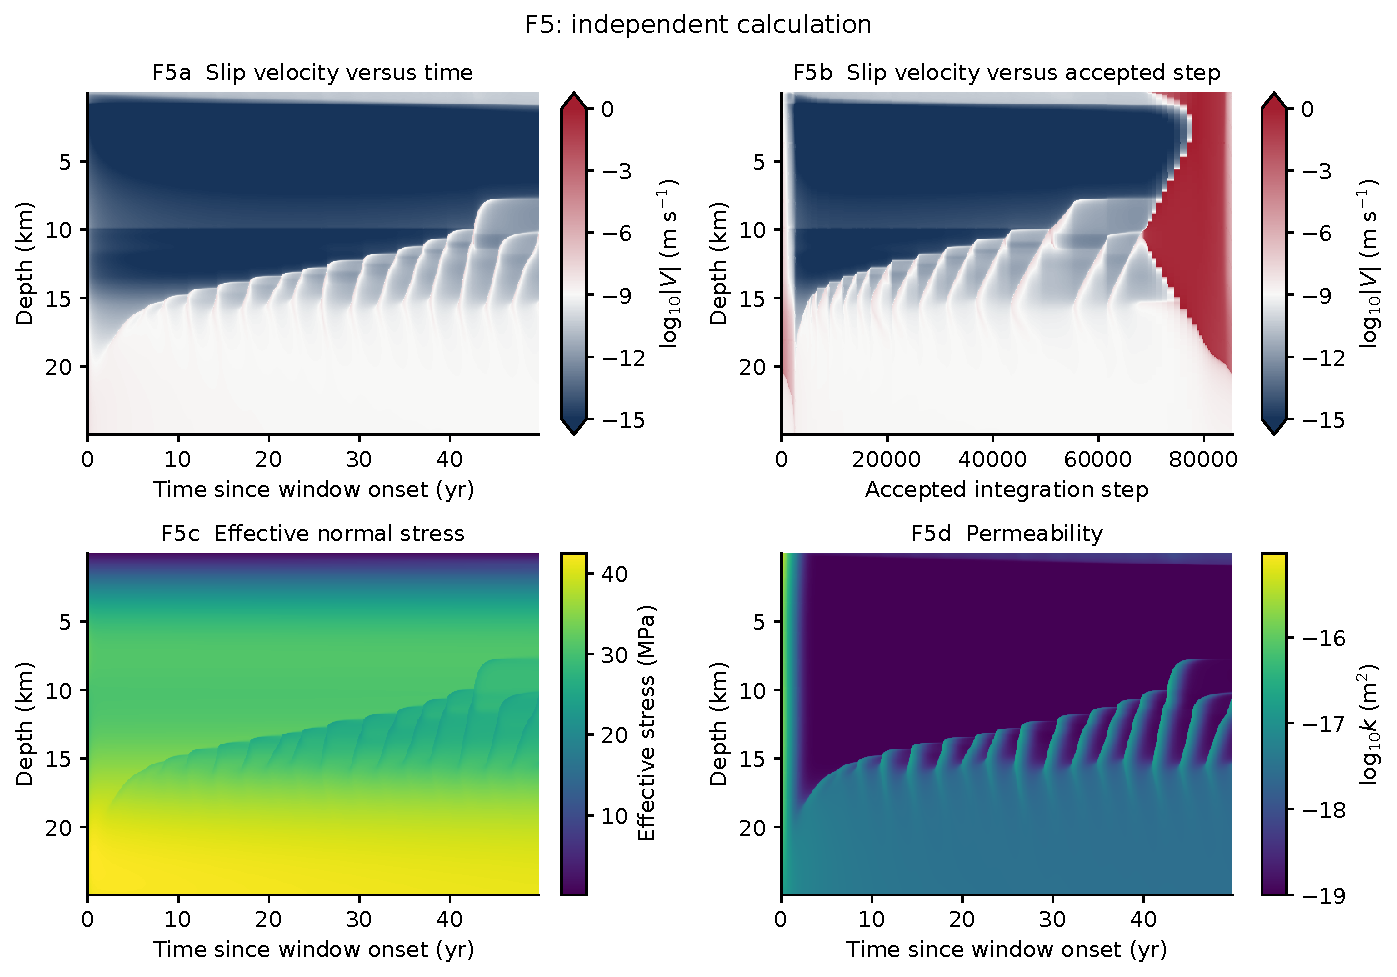
\includegraphics[width=\textwidth,height=.72\textheight,keepaspectratio]{../figures/F5.pdf}
\caption{Independent outputs corresponding to F5. F5a: Slip velocity versus time; F5b: Slip velocity versus accepted step; F5c: Effective normal stress; F5d: Permeability. Units and color scales are shown on the panels. Parameter files and selection rules are specified in the provenance sidecars. Cases: short (T=1e+07 s; coupled pressure). These panels are partial comparisons. Comparison target: Zhu et al.~\cite{zhu}.}\end{figure}
\clearpage\begin{figure}[p]\centering
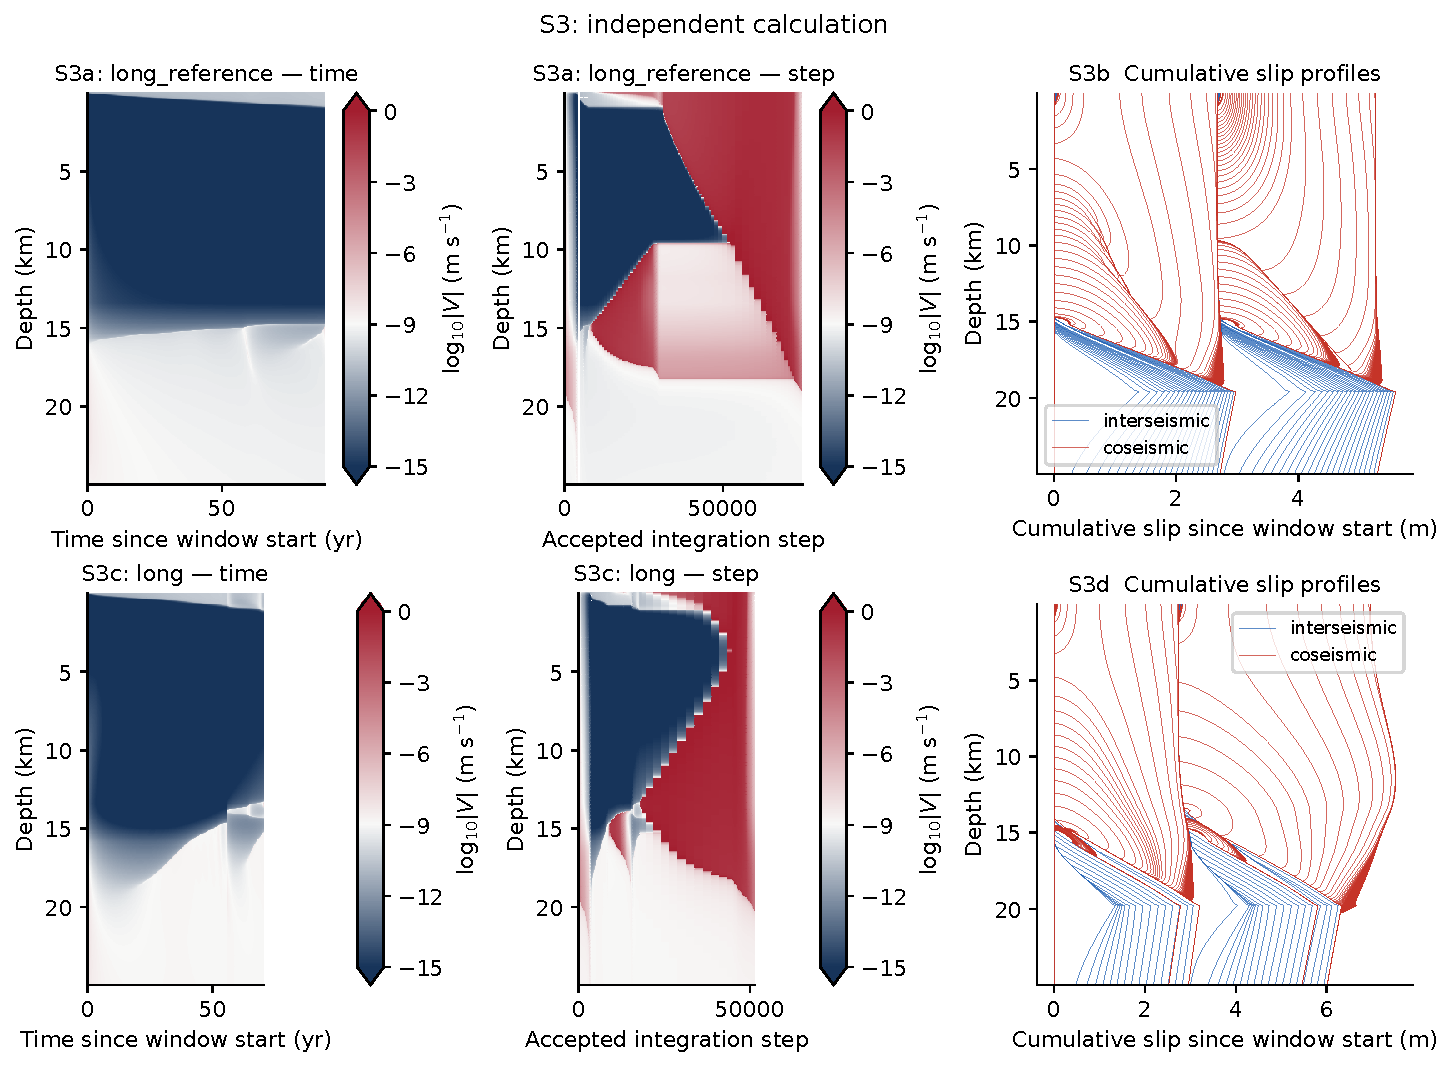
\includegraphics[width=\textwidth,height=.72\textheight,keepaspectratio]{../figures/S3.pdf}
\caption{Independent outputs corresponding to S3. S3a: Slip velocity in time and step coordinates; S3b: Cumulative slip profiles; S3c: Slip velocity in time and step coordinates; S3d: Cumulative slip profiles. Units and color scales are shown on the panels. Parameter files and selection rules are specified in the provenance sidecars. Cases: long (T=1e+09 s; coupled pressure), long\_reference (T=1e+09 s; fixed pressure). These panels are partial comparisons. Comparison target: Zhu et al.~\cite{zhu}.}\end{figure}
\clearpage\begin{figure}[p]\centering
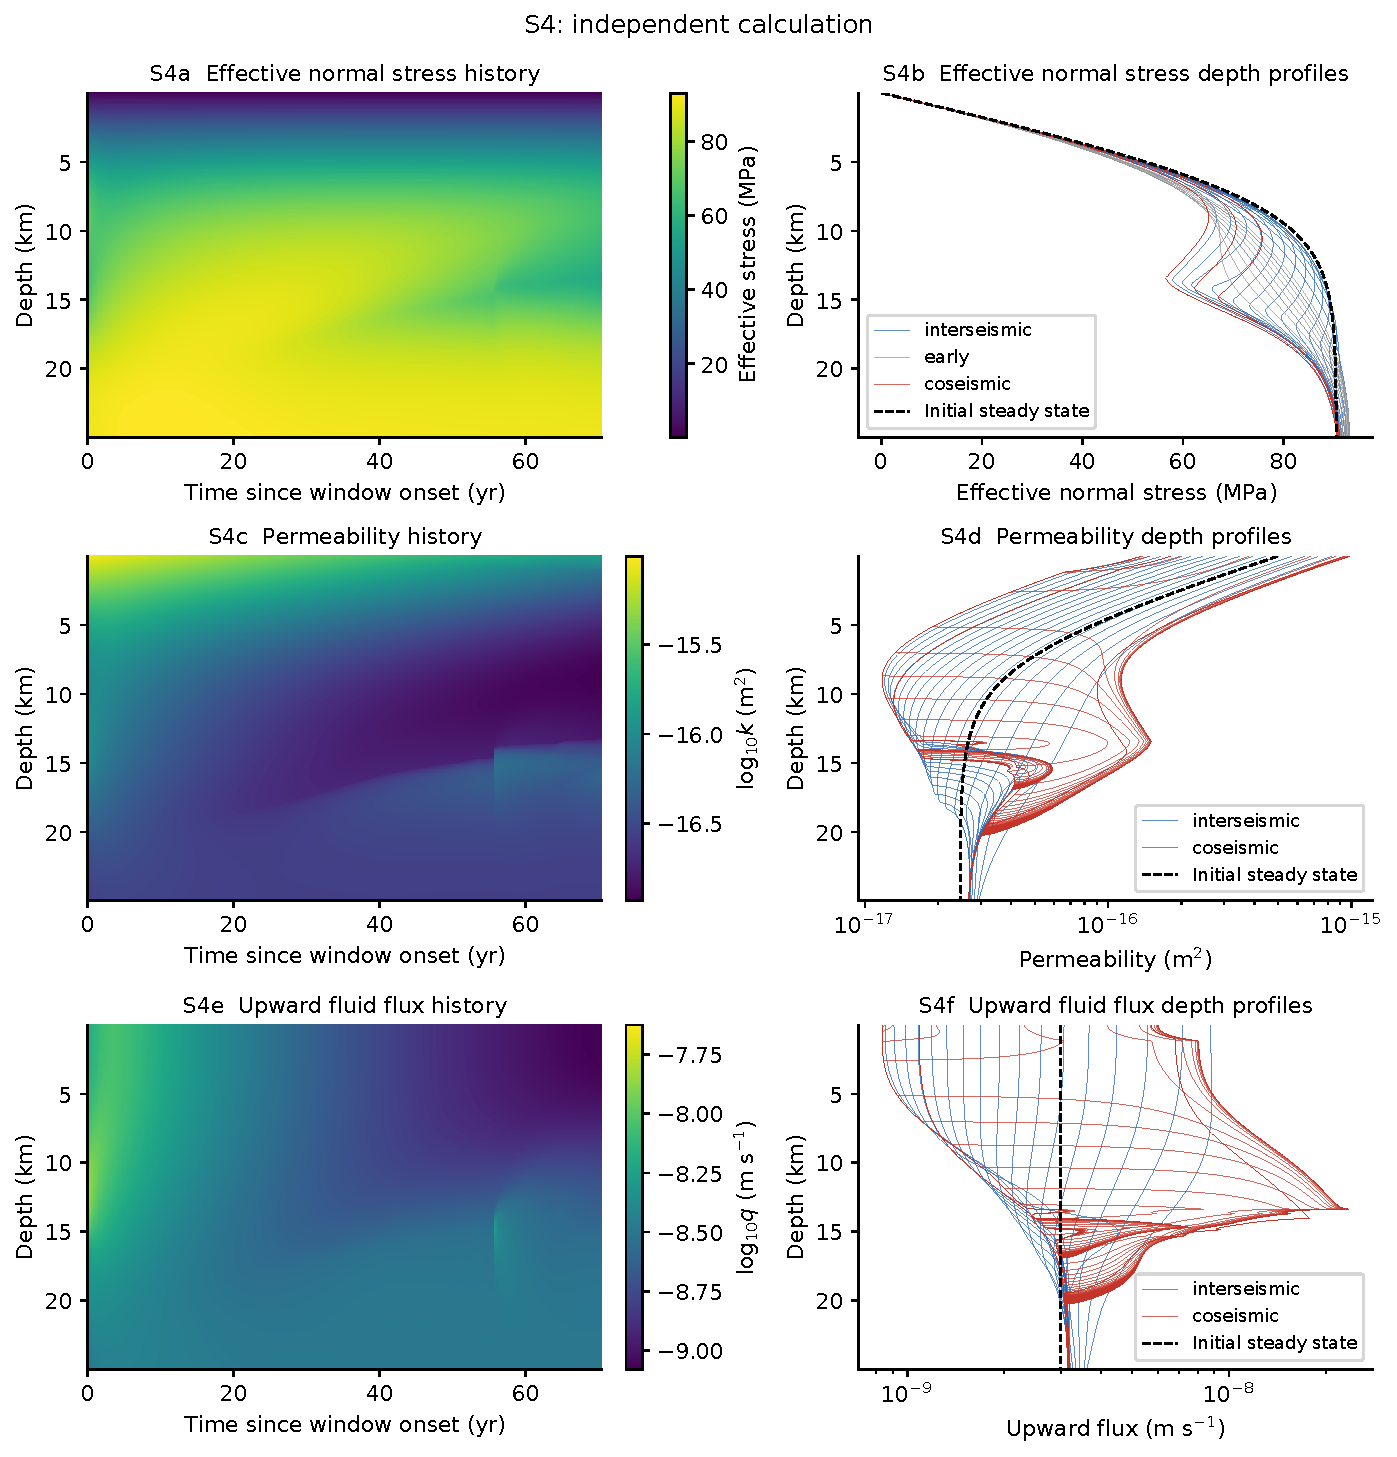
\includegraphics[width=\textwidth,height=.72\textheight,keepaspectratio]{../figures/S4.pdf}
\caption{Independent outputs corresponding to S4. S4a: Effective normal stress history; S4b: Effective normal stress depth profiles; S4c: Permeability history; S4d: Permeability depth profiles; S4e: Upward fluid flux history; S4f: Upward fluid flux depth profiles. Units and color scales are shown on the panels. Parameter files and selection rules are specified in the provenance sidecars. Cases: long (T=1e+09 s; coupled pressure). These panels are partial comparisons. Comparison target: Zhu et al.~\cite{zhu}.}\end{figure}
\clearpage\begin{figure}[p]\centering
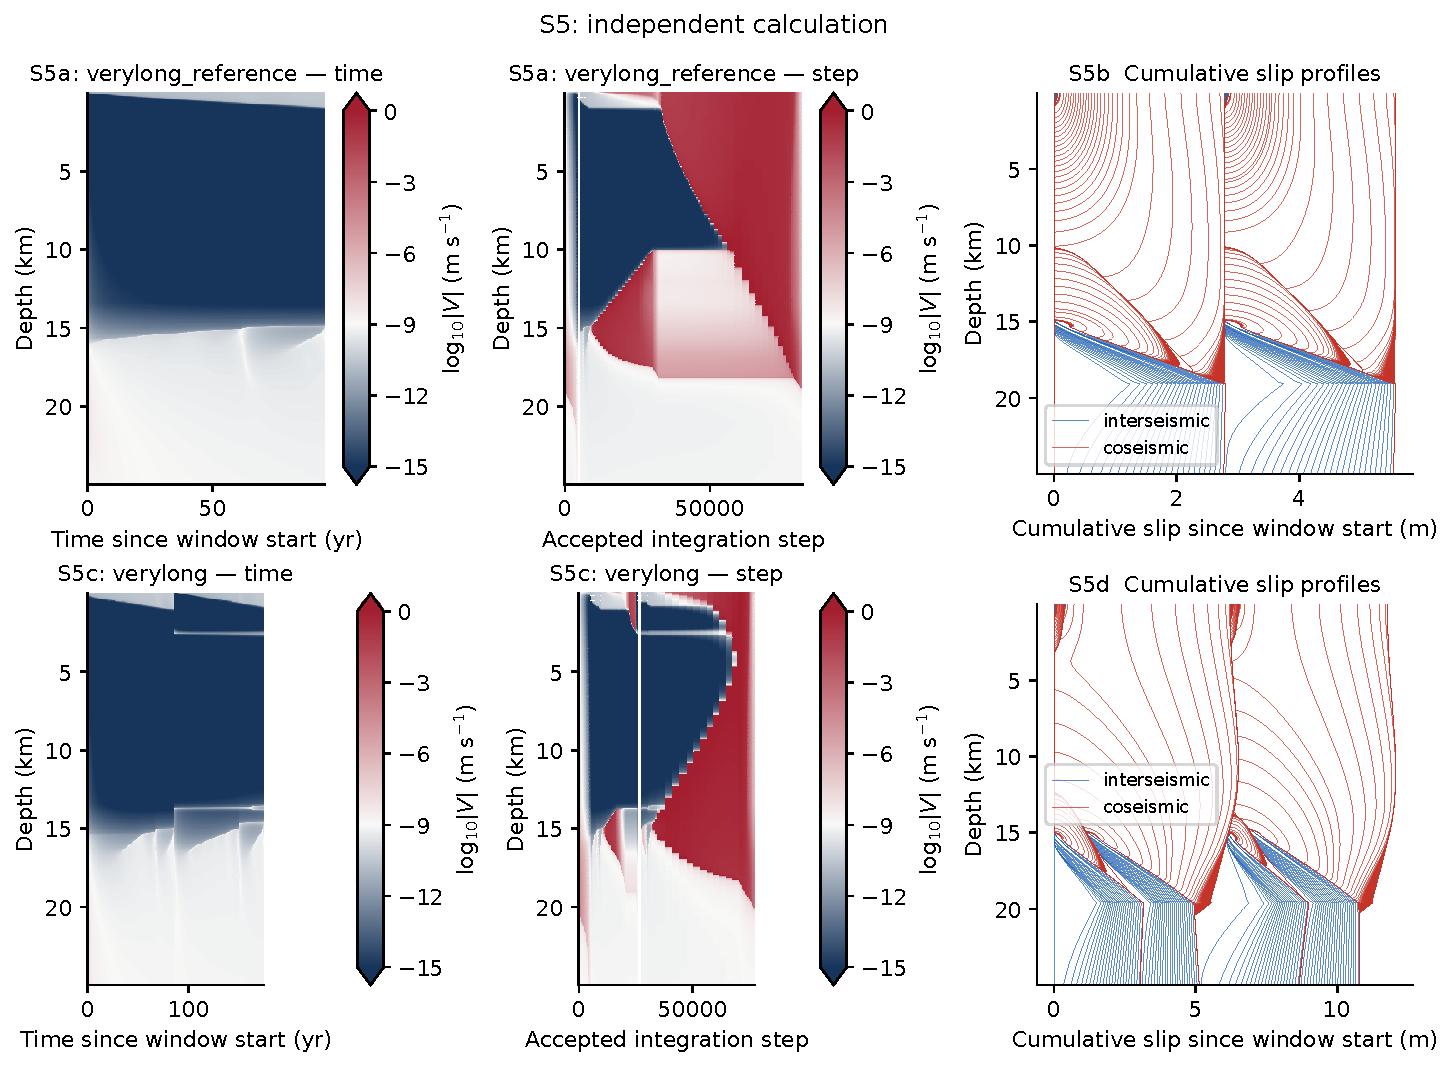
\includegraphics[width=\textwidth,height=.72\textheight,keepaspectratio]{../figures/S5.pdf}
\caption{Independent outputs corresponding to S5. S5a: Slip velocity in time and step coordinates; S5b: Cumulative slip profiles; S5c: Slip velocity in time and step coordinates; S5d: Cumulative slip profiles. Units and color scales are shown on the panels. Parameter files and selection rules are specified in the provenance sidecars. Cases: verylong (T=1e+10 s; coupled pressure), verylong\_reference (T=1e+10 s; fixed pressure). These panels are partial comparisons. Comparison target: Zhu et al.~\cite{zhu}.}\end{figure}
\clearpage\begin{figure}[p]\centering
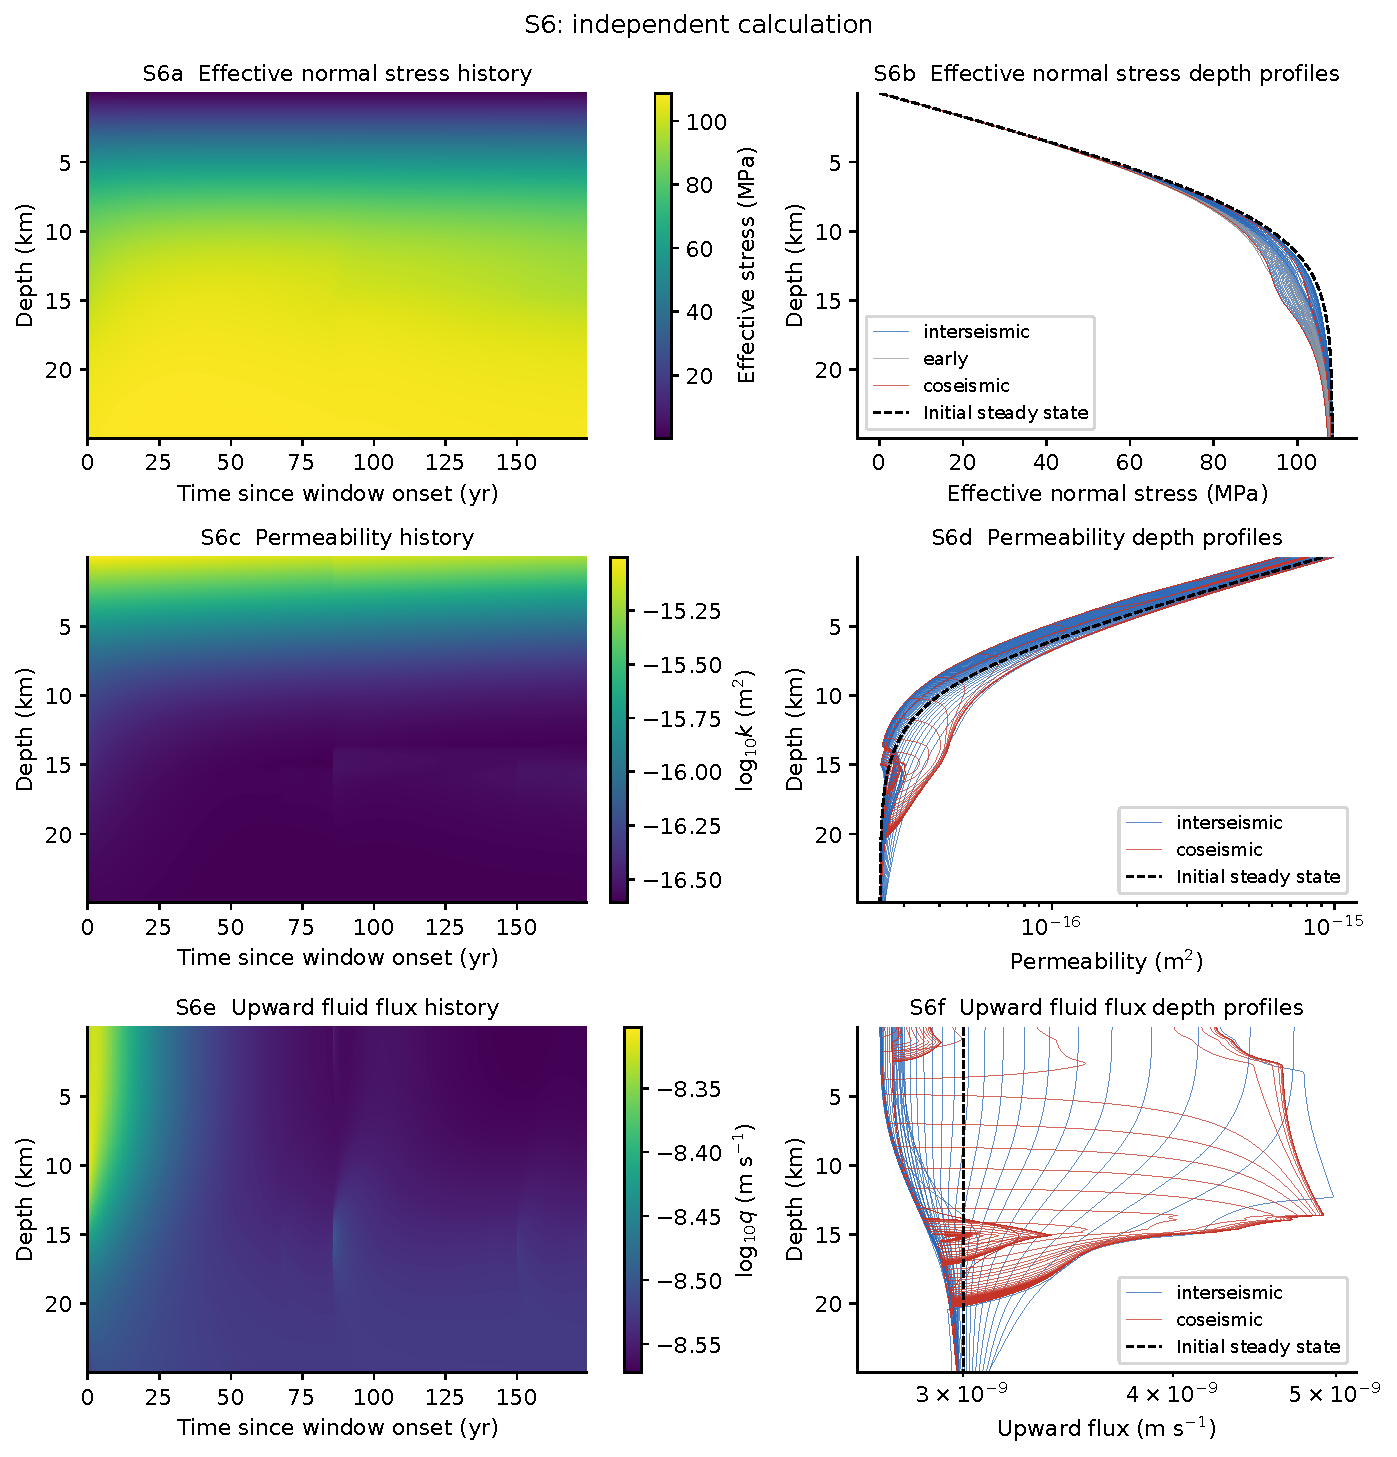
\includegraphics[width=\textwidth,height=.72\textheight,keepaspectratio]{../figures/S6.pdf}
\caption{Independent outputs corresponding to S6. S6a: Effective normal stress history; S6b: Effective normal stress depth profiles; S6c: Permeability history; S6d: Permeability depth profiles; S6e: Upward fluid flux history; S6f: Upward fluid flux depth profiles. Units and color scales are shown on the panels. Parameter files and selection rules are specified in the provenance sidecars. Cases: verylong (T=1e+10 s; coupled pressure). These panels are partial comparisons. Comparison target: Zhu et al.~\cite{zhu}.}\end{figure}

\clearpage
\section{Reproduction and remaining work}
The full project command builds and tests the C++ solver, runs all twelve cases,
extracts every panel, compiles the final report, and verifies its source bundle:
\begin{verbatim}
python3 -m pip install -r requirements.txt
python3 scripts/reproduce.py
\end{verbatim}
That full-duration run is ongoing at this snapshot. This interim report is
regenerated from completed, audited case metadata and generated panel packages:
\begin{verbatim}
python3 scripts/interim_report.py
\end{verbatim}
The command compiles \code{report/interim.pdf}, packages its standalone LaTeX
source and all included figures, and verifies compilation of the extracted bundle.
It records commands, exit codes, input hashes, and output hashes in
\code{data/interim_report_verification.json}. The source archive is
\code{report/interim-latex-source.zip}; the unexpanded source is already a single
file, \code{report/interim.tex}. All scientific arrays and their independent
generation commands are available in the repository.

Completion still requires the remaining calculations, the pending
panels, common-duration validation comparisons, the full scientific report,
visual and numerical artifact review, execution of the final regeneration
procedure, and publication of those final deliverables. This snapshot makes
the completed scientific results reviewable without declaring that work finished.
\begin{thebibliography}{9}
\bibitem{zhu} Zhu, W., K. L. Allison, E. M. Dunham, and Y. Yang (2020).
Fault valving and pore pressure evolution in simulations of earthquake sequences
and aseismic slip. \emph{Nature Communications}, 11, 4833.
\href{https://doi.org/10.1038/s41467-020-18598-z}{doi:10.1038/s41467-020-18598-z}.
Includes the published Supplementary Information.
\bibitem{allison} Allison, K. L., and E. M. Dunham (2018).
Earthquake cycle simulations with rate-and-state friction and power-law viscoelasticity.
\emph{Tectonophysics}, 733, 232--256.
\href{https://doi.org/10.1016/j.tecto.2017.10.021}{doi:10.1016/j.tecto.2017.10.021}.
\bibitem{kennedy} Kennedy, C. A., and M. H. Carpenter (2001).
Additive Runge--Kutta schemes for convection--diffusion--reaction equations.
NASA/TM-2001-211038, Appendix C.
\href{https://ntrs.nasa.gov/citations/20010075154}{NASA technical report}.
\end{thebibliography}

\end{document}
